\chapter{The Inquiry}

M. de Villefort kept the promise he had made to Madame Danglars, to
endeavor to find out how the Count of Monte Cristo had discovered the
history of the house at Auteuil. He wrote the same day for the required
information to M. de Boville, who, from having been an inspector of
prisons, was promoted to a high office in the police; and the latter
begged for two days time to ascertain exactly who would be most likely
to give him full particulars. At the end of the second day M. de
Villefort received the following note:

“The person called the Count of Monte Cristo is an intimate
acquaintance of Lord Wilmore, a rich foreigner, who is sometimes seen
in Paris and who is there at this moment; he is also known to the Abbé
Busoni, a Sicilian priest, of high repute in the East, where he has
done much good.”

M. de Villefort replied by ordering the strictest inquiries to be made
respecting these two persons; his orders were executed, and the
following evening he received these details:

“The abbé, who was in Paris only for a month, inhabited a small
two-storied house behind Saint-Sulpice; there were two rooms on each
floor and he was the only tenant. The two lower rooms consisted of a
dining-room, with a table, chairs, and side-board of walnut, and a
wainscoted parlor, without ornaments, carpet, or timepiece. It was
evident that the abbé limited himself to objects of strict necessity.
He preferred to use the sitting-room upstairs, which was more library
than parlor, and was furnished with theological books and parchments,
in which he delighted to bury himself for months at a time, according
to his valet de chambre. His valet looked at the visitors through a
sort of wicket; and if their faces were unknown to him or displeased
him, he replied that the abbé was not in Paris, an answer which
satisfied most persons, because the abbé was known to be a great
traveller. Besides, whether at home or not, whether in Paris or Cairo,
the abbé always left something to give away, which the valet
distributed through this wicket in his master’s name. The other room
near the library was a bedroom. A bed without curtains, four armchairs,
and a couch, covered with yellow Utrecht velvet, composed, with a
\textit{prie-Dieu}, all its furniture.

“Lord Wilmore resided in Rue Fontaine-Saint-Georges. He was one of
those English tourists who consume a large fortune in travelling. He
hired the apartment in which he lived furnished, passed only a few
hours in the day there, and rarely slept there. One of his
peculiarities was never to speak a word of French, which he however
wrote with great facility.”

The day after this important information had been given to the king’s
attorney, a man alighted from a carriage at the corner of the Rue
Férou, and rapping at an olive-green door, asked if the Abbé Busoni
were within.

“No, he went out early this morning,” replied the valet.

“I might not always be content with that answer,” replied the visitor,
“for I come from one to whom everyone must be at home. But have the
kindness to give the Abbé Busoni——”

“I told you he was not at home,” repeated the valet.

“Then on his return give him that card and this sealed paper. Will he
be at home at eight o’clock this evening?”

“Doubtless, unless he is at work, which is the same as if he were out.”

“I will come again at that time,” replied the visitor, who then
retired.

At the appointed hour the same man returned in the same carriage,
which, instead of stopping this time at the end of the Rue Férou, drove
up to the green door. He knocked, and it opened immediately to admit
him. From the signs of respect the valet paid him, he saw that his note
had produced a good effect.

“Is the abbé at home?” asked he.

“Yes; he is at work in his library, but he expects you, sir,” replied
the valet. The stranger ascended a rough staircase, and before a table,
illumined by a lamp whose light was concentrated by a large shade while
the rest of the apartment was in partial darkness, he perceived the
abbé in a monk’s dress, with a cowl on his head such as was used by
learned men of the Middle Ages.

“Have I the honor of addressing the Abbé Busoni?” asked the visitor.

“Yes, sir,” replied the abbé; “and you are the person whom M. de
Boville, formerly an inspector of prisons, sends to me from the prefect
of police?”

“Exactly, sir.”

“One of the agents appointed to secure the safety of Paris?”

“Yes, sir” replied the stranger with a slight hesitation, and blushing.

The abbé replaced the large spectacles, which covered not only his eyes
but his temples, and sitting down motioned to his visitor to do the
same. “I am at your service, sir,” said the abbé, with a marked Italian
accent.

“The mission with which I am charged, sir,” replied the visitor,
speaking with hesitation, “is a confidential one on the part of him who
fulfils it, and him by whom he is employed.” The abbé bowed. “Your
probity,” replied the stranger, “is so well known to the prefect that
he wishes as a magistrate to ascertain from you some particulars
connected with the public safety, to ascertain which I am deputed to
see you. It is hoped that no ties of friendship or humane consideration
will induce you to conceal the truth.”

“Provided, sir, the particulars you wish for do not interfere with my
scruples or my conscience. I am a priest, sir, and the secrets of
confession, for instance, must remain between me and God, and not
between me and human justice.”

“Do not alarm yourself, monsieur, we will duly respect your
conscience.”

At this moment the abbé pressed down his side of the shade and so
raised it on the other, throwing a bright light on the stranger’s face,
while his own remained obscured.

“Excuse me, abbé,” said the envoy of the prefect of the police, “but
the light tries my eyes very much.” The abbé lowered the shade.

“Now, sir, I am listening—go on.”

“I will come at once to the point. Do you know the Count of Monte
Cristo?”

“You mean Monsieur Zaccone, I presume?”

“Zaccone?—is not his name Monte Cristo?”

“Monte Cristo is the name of an estate, or, rather, of a rock, and not
a family name.”

“Well, be it so—let us not dispute about words; and since M. de Monte
Cristo and M. Zaccone are the same——”

“Absolutely the same.”

“Let us speak of M. Zaccone.”

“Agreed.”

“I asked you if you knew him?”

“Extremely well.”

“Who is he?”

“The son of a rich shipbuilder in Malta.”

“I know that is the report; but, as you are aware, the police does not
content itself with vague reports.”

“However,” replied the abbé, with an affable smile, “when that report
is in accordance with the truth, everybody must believe it, the police
as well as all the rest.”

“Are you sure of what you assert?”

“What do you mean by that question?”

“Understand, sir, I do not in the least suspect your veracity; I ask if
you are certain of it?”

“I knew his father, M. Zaccone.”

“Ah, indeed?”

“And when a child I often played with the son in the timber-yards.”

“But whence does he derive the title of count?”

“You are aware that may be bought.”

“In Italy?”

“Everywhere.”

“And his immense riches, whence does he procure them?”

“They may not be so very great.”

“How much do you suppose he possesses?”

“From one hundred and fifty to two hundred thousand livres per annum.”

“That is reasonable,” said the visitor; “I have heard he had three or
four millions.”

“Two hundred thousand per annum would make four millions of capital.”

“But I was told he had four millions per annum.”

“That is not probable.”

“Do you know this Island of Monte Cristo?”

“Certainly, everyone who has come from Palermo, Naples, or Rome to
France by sea must know it, since he has passed close to it and must
have seen it.”

“I am told it is a delightful place?”

“It is a rock.”

“And why has the count bought a rock?”

“For the sake of being a count. In Italy one must have territorial
possessions to be a count.”

“You have, doubtless, heard the adventures of M. Zaccone’s youth?”

“The father’s?”

“No, the son’s.”

“I know nothing certain; at that period of his life, I lost sight of my
young comrade.”

“Was he in the wars?”

“I think he entered the service.”

“In what branch?”

“In the navy.”

“Are you not his confessor?”

“No, sir; I believe he is a Lutheran.”

“A Lutheran?”

“I say, I believe such is the case, I do not affirm it; besides,
liberty of conscience is established in France.”

“Doubtless, and we are not now inquiring into his creed, but his
actions; in the name of the prefect of police, I ask you what you know
of him.

“He passes for a very charitable man. Our holy father, the pope, has
made him a knight of Jesus Christ for the services he rendered to the
Christians in the East; he has five or six rings as testimonials from
Eastern monarchs of his services.”

“Does he wear them?”

“No, but he is proud of them; he is better pleased with rewards given
to the benefactors of man than to his destroyers.”

“He is a Quaker then?”

“Exactly, he is a Quaker, with the exception of the peculiar dress.”

“Has he any friends?”

“Yes, everyone who knows him is his friend.”

“But has he any enemies?”

“One only.”

“What is his name?”

“Lord Wilmore.”

“Where is he?”

“He is in Paris just now.”

“Can he give me any particulars?”

“Important ones; he was in India with Zaccone.”

“Do you know his abode?”

“It’s somewhere in the Chaussée d’Antin; but I know neither the street
nor the number.”

\begin{figure}[ht]
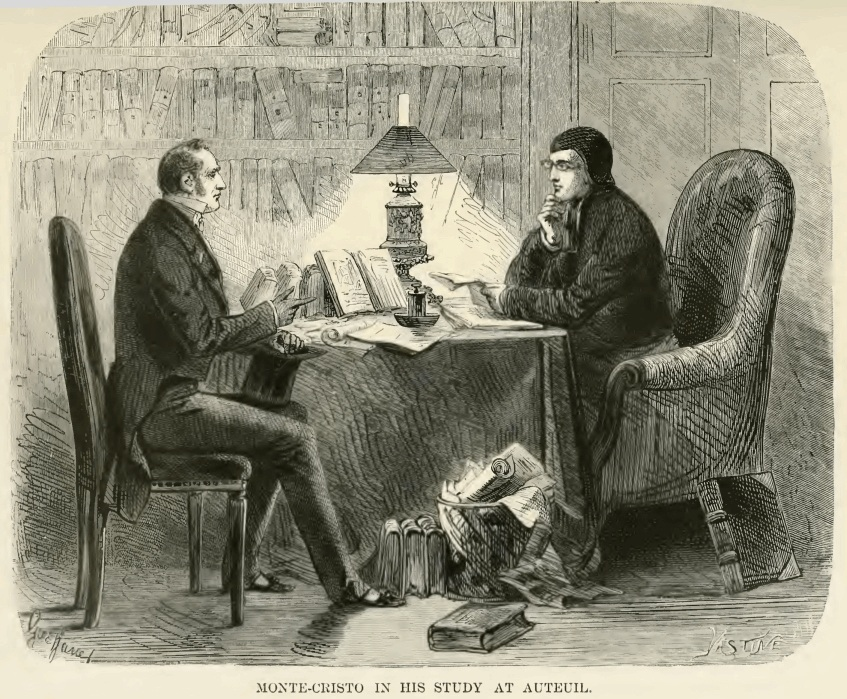
\includegraphics[width=\textwidth]{30289m.jpg}
\end{figure}

“Are you at variance with the Englishman?”

“I love Zaccone, and he hates him; we are consequently not friends.”

“Do you think the Count of Monte Cristo had ever been in France before
he made this visit to Paris?”

“To that question I can answer positively; no, sir, he had not, because
he applied to me six months ago for the particulars he required, and as
I did not know when I might again come to Paris, I recommended M.
Cavalcanti to him.”

“Andrea?”

“No, Bartolomeo, his father.”

“Now, sir, I have but one question more to ask, and I charge you, in
the name of honor, of humanity, and of religion, to answer me
candidly.”

“What is it, sir?”

“Do you know with what design M. de Monte Cristo purchased a house at
Auteuil?”

“Certainly, for he told me.”

“What is it, sir?”

“To make a lunatic asylum of it, similar to that founded by the Count
of Pisani at Palermo. Do you know about that institution?”

“I have heard of it.”

“It is a magnificent charity.” Having said this, the abbé bowed to
imply he wished to pursue his studies.

The visitor either understood the abbé’s meaning, or had no more
questions to ask; he arose, and the abbé accompanied him to the door.

“You are a great almsgiver,” said the visitor, “and although you are
said to be rich, I will venture to offer you something for your poor
people; will you accept my offering?”

“I thank you, sir; I am only jealous in one thing, and that is that the
relief I give should be entirely from my own resources.”

“However——”

“My resolution, sir, is unchangeable, but you have only to search for
yourself and you will find, alas, but too many objects upon whom to
exercise your benevolence.”

The abbé once more bowed as he opened the door, the stranger bowed and
took his leave, and the carriage conveyed him straight to the house of
M. de Villefort. An hour afterwards the carriage was again ordered, and
this time it went to the Rue Fontaine-Saint-Georges, and stopped at No.
5, where Lord Wilmore lived. The stranger had written to Lord Wilmore,
requesting an interview, which the latter had fixed for ten o’clock. As
the envoy of the prefect of police arrived ten minutes before ten, he
was told that Lord Wilmore, who was precision and punctuality
personified, was not yet come in, but that he would be sure to return
as the clock struck.

The visitor was introduced into the drawing-room, which was like all
other furnished drawing-rooms. A mantle-piece, with two modern Sèvres
vases, a timepiece representing Cupid with his bent bow, a mirror with
an engraving on each side—one representing Homer carrying his guide,
the other, Belisarius begging—a grayish paper; red and black
tapestry—such was the appearance of Lord Wilmore’s drawing-room.

It was illuminated by lamps with ground-glass shades which gave only a
feeble light, as if out of consideration for the envoy’s weak sight.
After ten minutes’ expectation the clock struck ten; at the fifth
stroke the door opened and Lord Wilmore appeared. He was rather above
the middle height, with thin reddish whiskers, light complexion and
light hair, turning rather gray. He was dressed with all the English
peculiarity, namely, in a blue coat, with gilt buttons and high collar,
in the fashion of 1811, a white kerseymere waistcoat, and nankeen
pantaloons, three inches too short, but which were prevented by straps
from slipping up to the knee. His first remark on entering was:

“You know, sir, I do not speak French?”

“I know you do not like to converse in our language,” replied the
envoy.

“But you may use it,” replied Lord Wilmore; “I understand it.”

“And I,” replied the visitor, changing his idiom, “know enough of
English to keep up the conversation. Do not put yourself to the
slightest inconvenience.”

“Aw?” said Lord Wilmore, with that tone which is only known to natives
of Great Britain.

The envoy presented his letter of introduction, which the latter read
with English coolness, and having finished:

“I understand,” said he, “perfectly.”

\begin{figure}[ht]
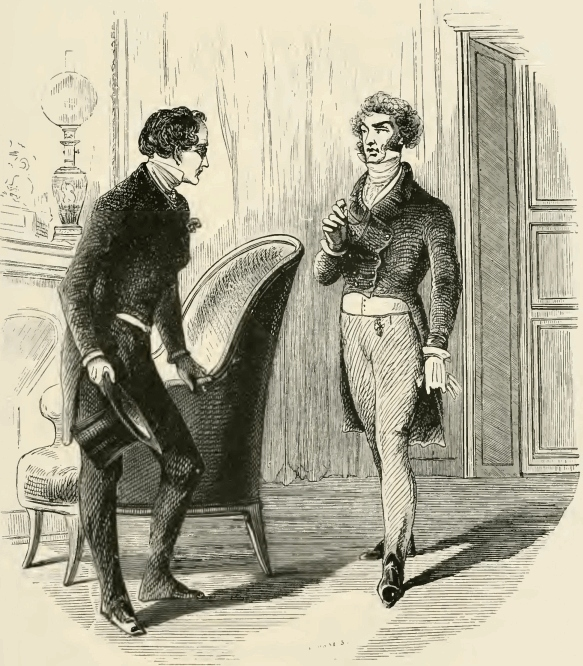
\includegraphics[width=\textwidth]{30293m.jpg}
\end{figure}

Then began the questions, which were similar to those which had been
addressed to the Abbé Busoni. But as Lord Wilmore, in the character of
the count’s enemy, was less restrained in his answers, they were more
numerous; he described the youth of Monte Cristo, who he said, at ten
years of age, entered the service of one of the petty sovereigns of
India who make war on the English. It was there Wilmore had first met
him and fought against him; and in that war Zaccone had been taken
prisoner, sent to England, and consigned to the hulks, whence he had
escaped by swimming. Then began his travels, his duels, his caprices;
then the insurrection in Greece broke out, and he had served in the
Grecian ranks. While in that service he had discovered a silver mine in
the mountains of Thessaly, but he had been careful to conceal it from
everyone. After the battle of Navarino, when the Greek government was
consolidated, he asked of King Otho a mining grant for that district,
which was given him. Hence that immense fortune, which, in Lord
Wilmore’s opinion, possibly amounted to one or two millions per
annum,—a precarious fortune, which might be momentarily lost by the
failure of the mine.

“But,” asked the visitor, “do you know why he came to France?”

“He is speculating in railways,” said Lord Wilmore, “and as he is an
expert chemist and physicist, he has invented a new system of
telegraphy, which he is seeking to bring to perfection.”

“How much does he spend yearly?” asked the prefect.

“Not more than five or six hundred thousand francs,” said Lord Wilmore;
“he is a miser.” Hatred evidently inspired the Englishman, who, knowing
no other reproach to bring on the count, accused him of avarice.

“Do you know his house at Auteuil?”

“Certainly.”

“What do you know respecting it?”

“Do you wish to know why he bought it?”

“Yes.”

“The count is a speculator, who will certainly ruin himself in
experiments. He supposes there is in the neighborhood of the house he
has bought a mineral spring equal to those at Bagnères, Luchon, and
Cauterets. He is going to turn his house into a \textit{Badhaus}, as the
Germans term it. He has already dug up all the garden two or three
times to find the famous spring, and, being unsuccessful, he will soon
purchase all the contiguous houses. Now, as I dislike him, and hope his
railway, his electric telegraph, or his search for baths, will ruin
him, I am watching for his discomfiture, which must soon take place.”

“What was the cause of your quarrel?”

“When he was in England he seduced the wife of one of my friends.”

“Why do you not seek revenge?”

“I have already fought three duels with him,” said the Englishman, “the
first with the pistol, the second with the sword, and the third with
the sabre.”

“And what was the result of those duels?”

“The first time, he broke my arm; the second, he wounded me in the
breast; and the third time, made this large wound.” The Englishman
turned down his shirt-collar, and showed a scar, whose redness proved
it to be a recent one. “So that, you see, there is a deadly feud
between us.”

“But,” said the envoy, “you do not go about it in the right way to kill
him, if I understand you correctly.”

“Aw?” said the Englishman, “I practice shooting every day, and every
other day Grisier comes to my house.”

This was all the visitor wished to ascertain, or, rather, all the
Englishman appeared to know. The agent arose, and having bowed to Lord
Wilmore, who returned his salutation with the stiff politeness of the
English, he retired. Lord Wilmore, having heard the door close after
him, returned to his bedroom, where with one hand he pulled off his
light hair, his red whiskers, his false jaw, and his wound, to resume
the black hair, dark complexion, and pearly teeth of the Count of Monte
Cristo.

It was M. de Villefort, and not the prefect, who returned to the house
of M. de Villefort. The procureur felt more at ease, although he had
learned nothing really satisfactory, and, for the first time since the
dinner-party at Auteuil, he slept soundly.
